% Chapter 3

\chapter{First version} % Main chapter title

\label{Chapter3} % For referencing the chapter elsewhere, use \ref{Chapter1} 


This chapter analyses which are the requirements of gAn Web at the first version and how they are implemented. This first version is very incomplete and aesthetically very raw, but very useful because it is meant to be a "test" to understand how to implement some functionalities and a base from which start to discuss with the super-users. 

\section{Functional requirements}
The definition of functional requirements aims to specifying in detail what the web application can do, and in which way an user can use it. The development of gAn Web is divided in three stages, so the requirements are peculiar and different for each stage. The first version (from now "gAn Web v1") is a very simple application: instead of access the program by a linux terminal like gAn, in gAn Web v1, the user can use the program through a graphical interface. 
The requirements of this version are the following:

\begin{enumerate}

% 1
\item The user, in the homepage, can choose the run (only one run, for the moment) in which he is interested, using an input field. This field has a validator, able to understand if the run number is inserted, if it is effectively a number, and if it is in an acceptable range. The user receives an explaining and precise error message directly on the homepage if the input field is empty or if the inserted value is not acceptable. Is it always possible validate the inserted run and ensure that the related Root file exists? No, because in some moments some sensors don't work properly and it is inevitable that some root files related to some runs are incomplete, or even in-existent. This problem will be solved in the next versions.

% 2
\item At this moment there is only a generic idea about what kind of analysis can be useful for the user, so in this version there will be only a generic analysis, able to dump in text all the possible information, and a group of example images (this is useless for the goal of the scientific research, but very useful to improve the understanding of the needed features of the web interface).
At this stage is not clear if the type of analysis will be chosen by the user of automatically selected by the program , so in gAn web v1 there are no buttons able to allow the user to select the type of analysis (this point will be reconsidered in next versions).

% 3
\item The user can start the program with a single click, by a button (usable only if the inserted number is valid).

% 4
\item When the program is executed the user can see the text output on the screen. This text is clear for a physicist (it is not clear for a person who doesn't have a specific preparation). This is an important point: there are big differences between the domain of the software engineering and the physics, so is better that this textual output is written by the hand of a physicist, to ensure to avoid misunderstanding due to different meanings assigned to symbols in different domains. Improve the legibility of the output will be a requirement for a more advanced version. 

% 5
\item When the program is executed the user can see the output images by clicking a button that link to an images-page. The images are ordered and organized by groups (the groups are related about which sensor takes the information necessary to create the image). The user can decide if he prefers to see the image in a little, medium or big format. The user can also decide if the images are distributed in the screen vertically or through a "carousel layout". The user can access the image in full-screen by clicking on it: he is redirected to a page with the image shown in full screen, and can return to the all-images page by a return button. It is absolutely important to understand exactly which information are interesting for the users, and show in the images only them and all of them, this point will be solved with a confrontation with the pilot-users. 

%6
\item The user can modify a configuration file (a .txt file on the server), by a web interface. In this file there are some values the need to be set (otherwise it uses default values), and the user can do it by radio buttons (in this way he is forced to choose valid values). This configuration file can modify the way in which gAn works and modify the resulting output (both the text and the images).   

\end{enumerate}

 
\section{Non-functional requirements}

This version (and actually also all the next versions) has some non-functional requisites:

\begin{enumerate}

\item The first is quite simple: gAn Web has to ensure that in case of crash of the program the web server mustn't crash too. The point is that on this web server (Apache server, installed on Linux) there are some other important applications, so, if gAn web crashes it is not a big problem, but the crash cannot force Apache, or worst the entire machine, to stop or restart. 
This requisite is quite easy to meet: a modern web application based on Html, Javascript, PHP and CSS is quite safe, a general crash of the server it is very unlikely to happen. If the C++ application or some Root libraries crashes (for example if the user asks for an inexistent run) the web application gracefully warn the user about the problem, but without uncontrolled behaviors.  

\item The application must work without install nothing. Also this requirement is very easy to meet: gAn Web is a web interface, it requires only a browser, nothing else.

\item The application must be compatible with any machine (except mobile phones, not requested), regardless of hardware, operating system, installed software. Also this requirement is achieved because of gAn Web only needs a browser to be used. A good observation is that the application is typically used on the computers of the AEgIS control room, that have a quite big screens, but to be sure is better to create an application able to adapt itself also to (quite) little screens.  

\item The application must be easy to be modified and extended in the future by persons who aren't necessarily software engineers. The point is that the student who wrote this program is a "momentary collaborator" in the AEgIS experiment, and all the modifications to the program must be done by other people, in most cases physicists. So the best way is to comment in detail the code and keep the code simple (this is a basic good-programming requirement).   


\end{enumerate}

\section{Scenario based functional analysis}

Following there are a list of scenarios in which a user achieves a goal by doing a list of steps. The goal of these scenarios is to show in detail how the interaction between the user and the system takes place. In this first version, the complexity of the scenarios is very low. 

\begin{enumerate}

\item The user in interested in the run 31111. In particular he is interested in the peak (the highest value) reached by a sensor named Mimito (this kind of task is very common). At this stage we still not work with kinds of analysis. The user, opened a browser in the homepage, inserts the run number and push "Send". He waits some seconds (there is a progress bar) and he arrives in a textual output page. At this point he can search in the text the information in which he is interested (it is a numerical value). Probably he is interested also in a image, to understand spatially where this peak is: he clicks on the "Show Images" button, he goes in the images pages, he selects the group "mimito", and the browser shows him a png image showing an histogram in 3 dimension: on the z-axis there is the peak, he can understand in which place (identified by x-axis and y-axis coordinates), the peak takes place, and how is shaped the resulting 3-d figure. From there he can return to the homepage and do another task.   

\item The user is no more interested in Mimito, but in another sensor: Faraday Cup. The user wants to know what are the values detected by the sensor in the same run (also this scenario is very common, often when the result of a sensor is unexpected, checking the others is interesting). This other sensor is not automatically enabled, so the user goes through the "Edit Configuration" button in a page able to modify the configuration file. Here the user can see a list of sensors, and he can use radio-buttons to modify their values from no (==disabled), to yes (==enabled). The user enables all the sensors, confirms the changes, and automatically returns in the homepage. Now he can like before insert the number, and get the outputs in textual and in images format.  



\end{enumerate}


\section{Prototyping}

This version is very simple and it contains only the basic functionalities. 
The goal of this version are: to understand if this kind of system can be useful for the users, and to experiment some technical solutions to create the features needed to achieve the goals. 

To create a prototype in this case the web programming is preferred on programs able to produce mock-ups, because the designer is quite expert in web development and can produce it quite rapidly, but he is not used to produce mock-ups with specialized software so the production of mock-ups would be slower than the complete development (actually, quite complete). 


Following are visible some part of the first prototype, with very simple features.

\begin{enumerate}
\item The homepage:

\begin{figure}[H]
\centering
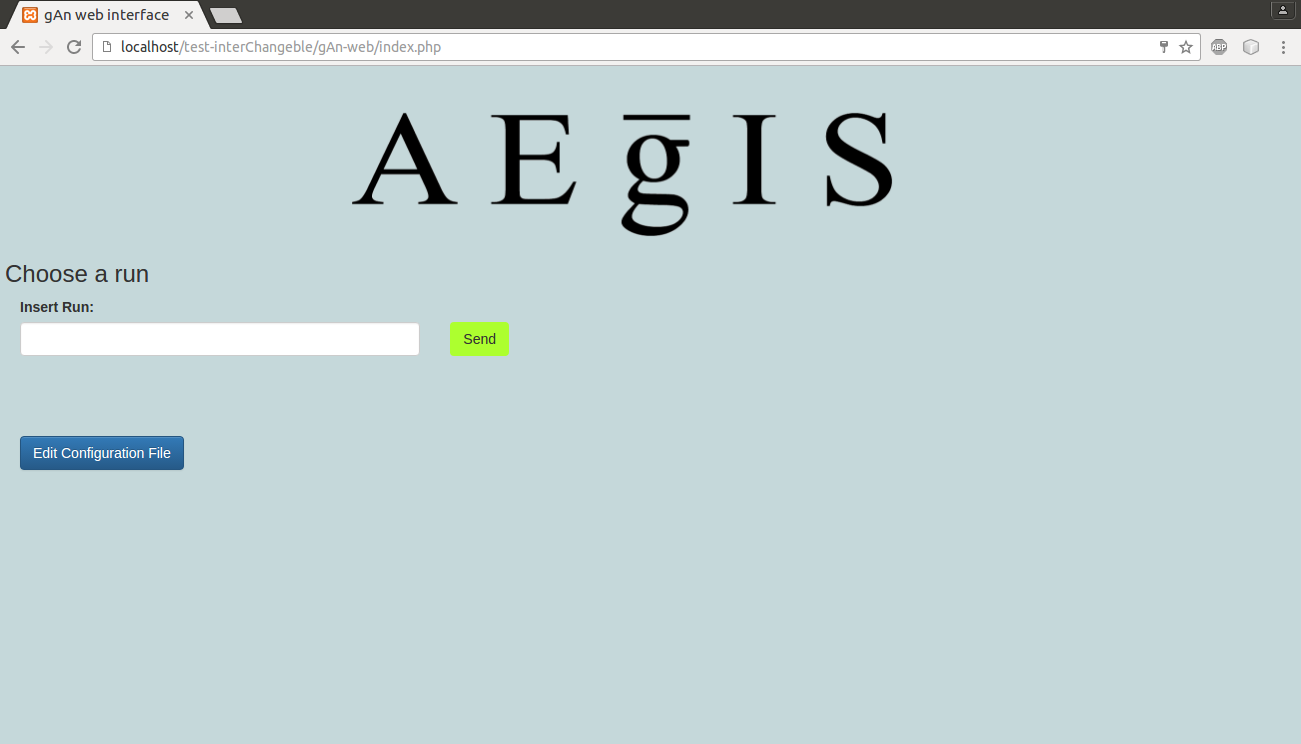
\includegraphics[scale=0.25]{HomePageOLD.png} 
\caption{First version: the first homepage of gAn Web}
\end{figure}

It is quite clear: There is the AEgIS Logo, an input field where the user can insert a run number (only one in this version) and a "Send" button to start the analysis (using gAn). A button "Edit Configuration File" allows the user to  enter in the page dedicated to the configuration of the program.

\item The text output page:

\begin{figure}[H]
\centering
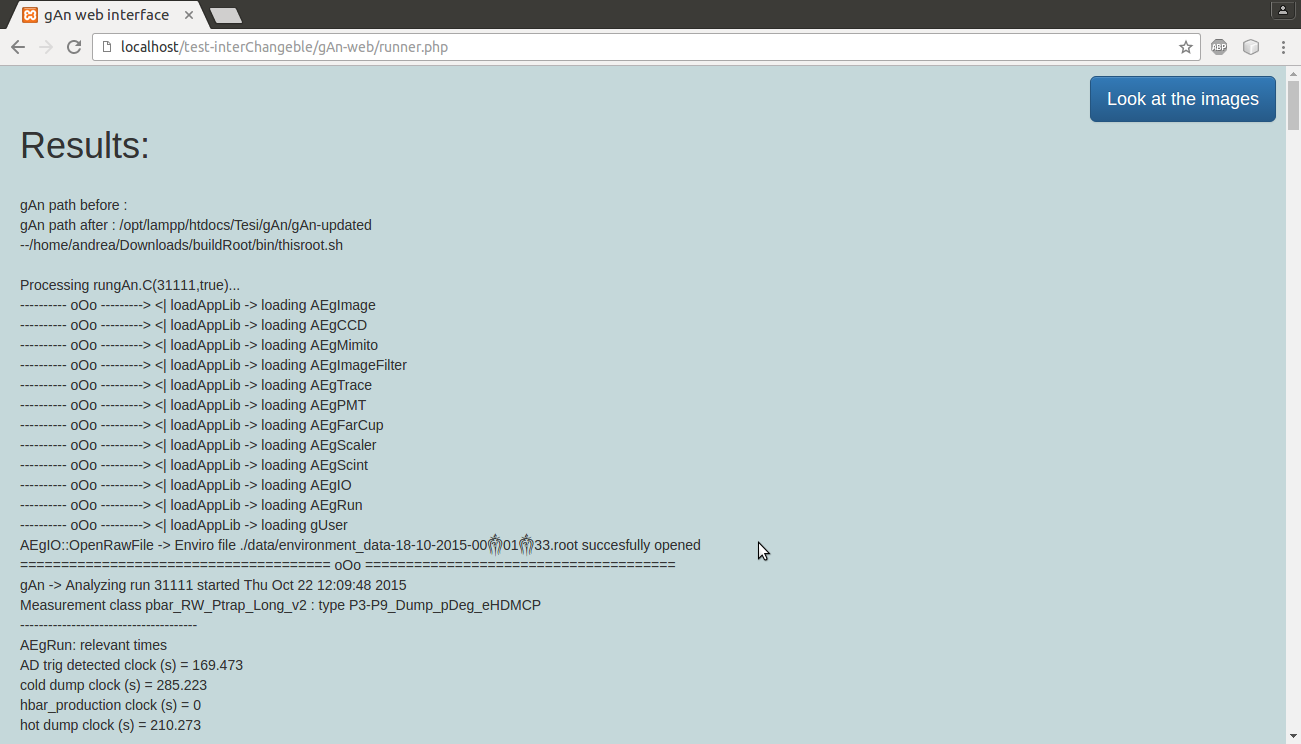
\includegraphics[scale=0.25]{TextOutputOLD.png} 
\caption{First version: the page related to the textual output of gAn Web}
\end{figure}
  
The textual result of the computation is visible: it seems to be too long and incomprehensible, but for physicists it is quite clear; to understand what is the best way to format this output a further confrontation with the users is needed. The graphics is very minimalist, there is only one button: "Look at the images", that sends the user to the page related to the images. 



\item The page related to the images:

\begin{figure}[H]
\centering
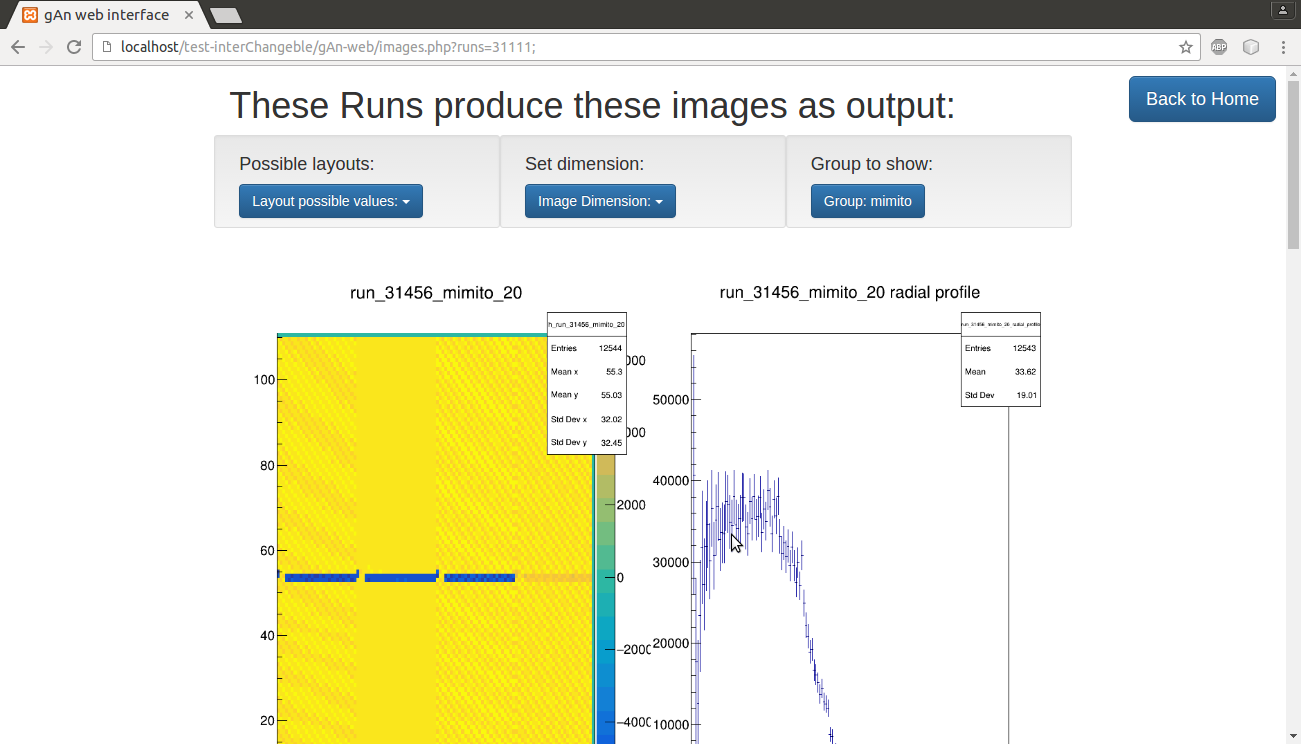
\includegraphics[scale=0.25]{AllImagesPageOLD.png}
\caption{First version: the page able to show the output images in the early prototype}
\end{figure}   

This page shows the images in a dynamic framework, that the user can edit.
The user can choose by dropdown menus the dimension, the layout ("vertical", if he prefers the images disposed vertically one above the other, "carousel" if he prefers the images organized horizontally, navigable by a "next" button and a "previous" button), the group to show (each image belongs to a group, each group usually is composed by 2-3 images). Clicking on a image the user can open it in a full page version (but it is still a static image, a png).


\item The page that aims to edit the configuration file:

\begin{figure}[H]
\centering
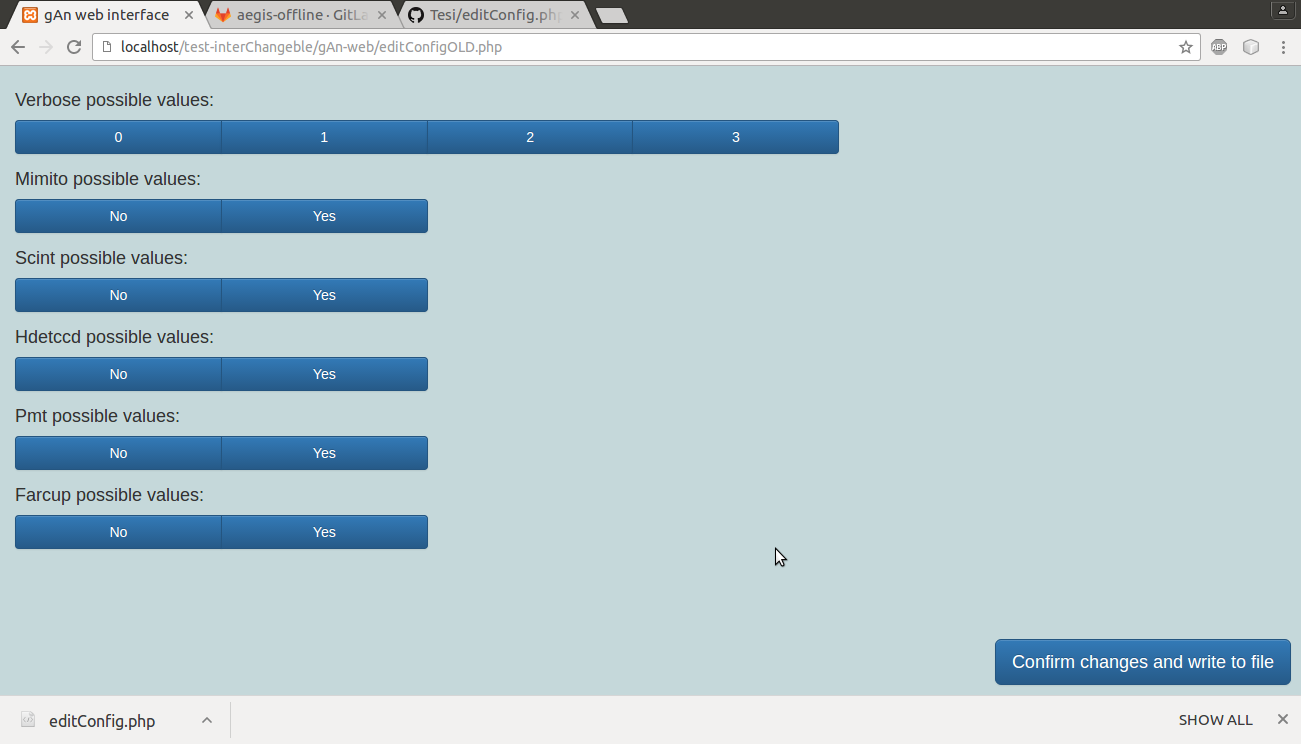
\includegraphics[scale=0.25]{EditConfigOLD.png}  
\caption{First version: the configuration page}
\end{figure}   

This page allows the user to choose by radio buttons (modified using Bootstrap graphic) the value to insert in the configuration file of gAn. Radio buttons force users to insert correct values.    

\end{enumerate}

\section{How the early version can be improved}
The early version's goal is just to be a demo. In particular, it is based on the assumption that the user knows in every moment all about gAn (how does it work,  what is the meaning of each field of the configuration file, and so on). It can be improved literally in every point, according with the principles of the Human Computer Interaction.

